\chapter{Deep Generative Models}
\section{Variational Autoencoder}

Our goal is to find the data distribution $p(X)$. \Cref{fig:dgm} represents a general structure of deep generative model. As you can see, we first sample $z\sim p(z)$ and feed it into a deep neural network $f(z)$ and output $x$.

\begin{figure}[h]
	\begin{center}
		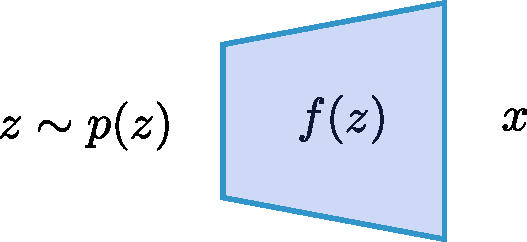
\includegraphics[scale=0.5]{./images/dgm.pdf}
	\end{center}
	\caption{General structure of deep generative models. This model does not infer $z$ from $x$.}
	\label{fig:dgm}
\end{figure}

VAE performs an inference by introducing a probabilistic encoder, called inference network. VAEs are generative model with a latent variable distributed according to some distribution $p(z_i)$. The observed variable is distributed according to a conditional distribution 
$$p_\theta(x_i|z_i)$$
This conditioning means the latent variable values are the one most likely given the observations. We also create a distribution $q_\phi(z_i|x_i)$. We would like to be able to encode our data into the latent variable space. Let's model the distribution.

\begin{itemize}
	\item $p_\theta(x_i|z_i)\sim \mathcal{N}(x_{i}|\mu(z_i), \sigma^2(z_i))$: A probabilistic decoder (or generative network, $\theta$)
	\item $q_\phi(z_i|x_i)$: A probabilistic encoder (or inference network $\phi$). We can choose a family of distributions for our conditional distribution $q$ (\eg standard Gaussian distribution). 
		$$q_\phi(z_i|x_i) = \mathcal{N}(z_i|\mu(x_i, W_1), \sigma^2(x_i, W_2)I),$$
	where $W_1$ and $W_2$ are network weights and collectively denoted as $\phi$. We create a neural network to model the distribution $q$ from our data in a non-linear manner. The outputs of the network are $\mu$ and $\sigma$. 
\end{itemize}

\begin{figure}[h]
	\begin{center}
		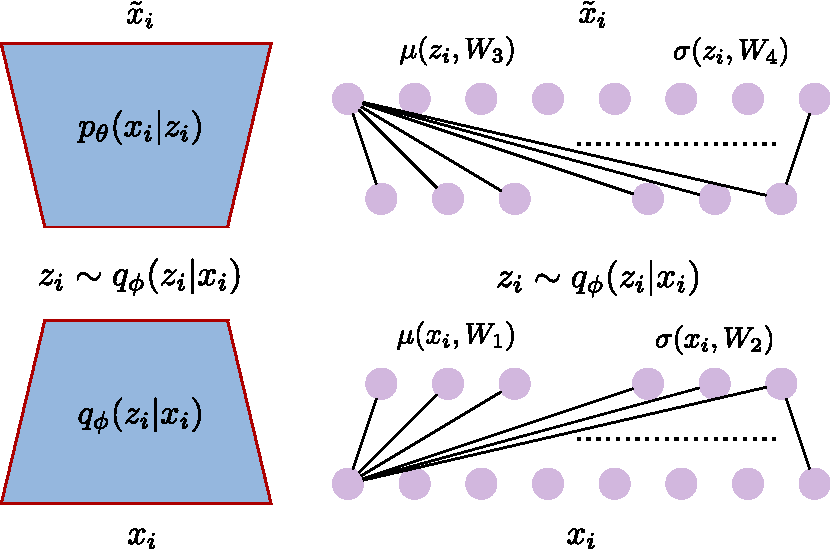
\includegraphics[scale=0.5]{./images/encoder.pdf}
	\end{center}
	\caption{Overview of variational autoencoder.}
	\label{fig:vae}
\end{figure}



\begin{align*}
	p(X,Z|\theta) &=  \prod_{i=1}^{n}\underbrace{p(x_i|z_i,\theta)}_{\textrm{Likelihood, Generator}}\underbrace{p(z_i|\theta)}_{\textrm{Prior on latent variable}}\\
	&= \prod_{i=1}^{n} \mathcal{N}(x_{i}|\underbrace{\mu(z_i), \sigma^2(z_i)}_{\textrm{Non-linear}}) \mathcal{N}(z_i|0, I)
\end{align*}

Subsequently, marginal distributions can be expressed as follows under i.i.d. assumption:
\begin{align*}
	p(X|\theta) &= \prod_{i=1}^{n} p(x_i|\theta) \\
	&= \prod_{i=1}^{n} \int p(x_i, z_j|\theta) dz_j \\
	& = \prod_{i=1}^{n} \int p(x_i|z_i, \theta)p(z_i|\theta)dz_i \\
	& = \prod_{i=1}^{n} \int \mathcal{N}(x_{i}|\mu(z_i), \sigma^2(z_i)) \underbrace{\mathcal{N}(z_i|0, I)}_{\textrm{Mixture weight}} dz_i
\end{align*}

\begin{itemize}
	\item As you can see, the marginal distribution $p(X|\theta)$ becomes a mixture of Gaussian (infinite mixture of Gaussian). 
	\item Even though $p(x|z)$ and $p(z)$ are normal, $p(x)$ is not normal, because it is a mixture distribution.
	\item The non-linearity of Gaussian parameters (modeled by a neural network), conjugacy between the prior and the likelihood does not hold anymore.
%	\item Diagonal covariance matrix does not mean the independence between elements of $x$.
	\item Again, $\mu$ and $\sigma$ is non-linear function of $z$ modeled by some non-linear neural network. The neural network works as a powerful non-linear parameter approximator (based on universal approximation theorem). 
	\item Simple prior is used. Let's consider the data $x$ is an image of $100\times 100$ pixels. Then the covariance matrix has to be $10000\times 10000$. Thus, it is common to set a simple prior such as the standard Gaussian (covariance matrix is diagonal matrix). However, even if we set a simple distribution, with the infinite mixture of Gaussian, we can model any distribution.
	\item VAE uses a global parametric model to predict the local
		variational parameters for each data point (amortized inference). 
%	\item Under the simple standard Gaussian prior assumption, the generator, $p(x_i|z_i,\theta)$, returns factorized Gaussian whose mean and variance are non-linear functions of latent variable modelled by deep neural network parameterized by $\theta$.
%	$$p(x_i|z_i,\theta) = \mathcal{N}(x_{i}|\mu(z_i), \sigma^2(z_i))$$
%	\item VAEs uses a simple prior over latent variables and complicated and powerful generator (neural network).
	\item It allows to convert complicated large-dimensional data distributions into simple lower-dimensional latent variable representations.  
%	\item $Std = e^{\frac{1}{2}\log (Var)}$, thus output is the log var
\end{itemize}

%\footnotetext[1]{Uncorrelated relationship does not imply the independence (independence makes covariance to be diagonal). If two variables are uncorrelated, $Cov(x_i,x_j)=0 $, there is no linear relationship between them.}
%\footnotetext[2]{In practice, simple prior could be a problem.}
